% Template for EUSIPCO-2012 paper; to be used with:
%          spconf.sty  - LaTeX style file, and
%          IEEEbib.bst - IEEE bibliography style file.
% --------------------------------------------------------------------------
\documentclass{article}
\usepackage{spconf,amsmath,graphicx}
\usepackage{tikz}
\usepackage{amsmath}
\usetikzlibrary{calc,snakes}
\usetikzlibrary{shapes,snakes}
\usetikzlibrary{calc,chains,positioning}
\usepackage{cases}
\usepackage{phaistos}
%%%%%\usepackage{flushend}

% Example definitions.
% --------------------
\def\x{{\mathbf x}}
\def\L{{\cal L}}

\def\baselinestretch{.9}

% Title.
% ------
\title{THE EFFECT OF INVERSE FILTER LENGTH ON THE ROBUSTNESS \\ OF ACOUSTIC MULTICHANNEL EQUALIZATION}
%
% Single address.
% ---------------
\name{Ina Kodrasi, Simon Doclo}
\address{
%email of first author
%affiliation and address of first author
University of Oldenburg, Institute of Physics, Signal Processing Group, Oldenburg, Germany \\
{\tt \char123 ina.kodrasi,simon.doclo\char125 @uni-oldenburg.de}\\
%affiliations of remaining authors
}


\begin{document}

\maketitle
%
\begin{abstract}
\vspace{-0.1cm}
In acoustic multichannel equalization techniques, generally the length of the inverse filters is chosen such that exact inverse filters can be designed for perfectly estimated room impulse responses~(RIRs).
However, since in practice the estimated RIRs typically differ from the real RIRs, this choice of the inverse filter length may not be optimal.

This paper investigates the effect of the inverse filter length on the robustness of acoustic multichannel equalization.
A mathematical link between the inverse filter length and robustness to channel estimationg errors is provided.
Experimental results for speech dereverberation show that using shorter inverse filters yields similar or higher performance for all considered multichannel equalization techniques, while reducing the computational complexity of the inverse filter design.
\end{abstract}
%
\begin{keywords}
acoustic multichannel equalization, robustness, channel estimation errors, dereverberation
\end{keywords}
%

\vspace{-0.1cm}
\section{Introduction}
\label{sec:intro}
\vspace{-0.2cm}

In teleconferencing applications, voice-controlled systems, and hearing aids, the recorded speech signals are often corrupted by reverberation, resulting in a distant and spectrally distorted sound. 
In order to mitigate the effects of reverberation, several approaches have been developed which can be broadly classified into speech enhancement and acoustic multichannel equalization techniques~\cite{Naylor_Derev_book}.
Speech enhancement techniques such as the linear prediction~\cite{Gaubitch_EUSIPCO_2004} or the spectral subtraction approaches~\cite{Habets2009a} directly exploit the effects of reverberation on the recorded speech, whereas multichannel equalization techniques are based on estimating and inverting the room impulse responses~(RIRs) between the source and the microphone array~\cite{Miyoshi_ITASS_1988, Kodrasi_ICASSP_2012}. 

A well-known multichannel equalization technique is the multiple-input/output inverse theorem (MINT) which aims to recover the anechoic speech signal~\cite{Miyoshi_ITASS_1988}. 
However, such an approach has been shown to be very sensitive to small fluctuations in the estimated RIRs, resulting in severe distortions in the output signal~\cite{Radlovic_ITSA_2000}.
In order to increase the robustness to channel estimation errors, partial multichannel equalization techniques such as relaxed multichannel least-squares~(RMCLS)~\cite{Zhang_IWAENC_2010}, channel shortening~(CS)~\cite{Kallinger_ICASSP_2006}, and partial multichannel equalization based on MINT~(P-MINT)~\cite{Kodrasi_ICASSP_2012} have been investigated, which aim to shorten the overall impulse response such that only the reverberant tail is suppressed.
While RMCLS and CS put no constraints on the remaining direct path and early reflections, the P-MINT approach is perceptually advantageous since it aims to also control the remaining filter coefficients~(i.e. direct path and early reflections) after shortening.
In~\cite{Kodrasi_ICASSP_2012} and~\cite{Zhang_IWAENC_2010} it has been experimentally validated that such a relaxed constraint for designing inverse filters as compared to complete channel equalization leads to a significant increase in robustness in the presence of channel estimation errors. 

The length of the inverse filters in all aforementioned techniques has been conventionally chosen such that exact inverse filters can be constructed for perfectly estimated RIRs.
In this paper, the effect of the filter length on the performance/robustness of acoustic multichannel equalization is investigated.
It is shown that using a shorter inverse filter than conventionally used increases robustness to estimation errors as well as makes the inverse filter design computationally more efficient.

\vspace{-0.1cm}
\section{Acoustic Multichannel Equalization}
\label{sec: intro}
\vspace{-0.2cm}

Consider an acoustic system with a single source and $M$ microphones as depicted in Fig.~\ref{fig: acsys}.
\begin{figure}[b]
  \centering
  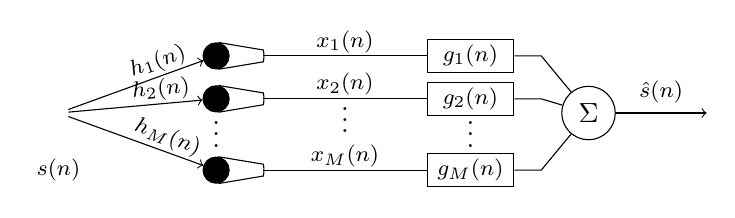
\begin{tikzpicture}
    % Adjustments
    \def\micd{.1cm}                % mic diameter
    \def\micl{.6cm}                % mic length
    \def\micw{.15cm}                % mic width
    \def\micbend{10}               % mic bottom bend
    \def\micdistance{.2cm}         % distance between microphones
    \def\filterdistance{2.5cm}     % distance between microphone and filter
    \def\filteroutline{.9cm}       % length of line which gets out of filter
    \def\sumdistance{1.5cm}        % distance of sum node to the filter
    \def\sumoutline{1cm}           % length of line which gets out of sum
    \def\headdistance{2cm}         % distance between microphone and head

    % Styles
    \tikzset{%
      mic head/.style={fill=black,draw=black,circle,minimum size=\micd},
      filter/.style={draw,minimum width=1.1cm,inner sep=2pt},
      sum/.style={draw,circle},
      xlabel/.style={inner sep=1pt,above,midway},
      sumlabel/.style={xlabel},
      hlabel/.style={xlabel,sloped,pos=.7},
      head/.style={font=\Large}
    }

    % Draw Microphones
    \begin{scope}[start chain=going below,every node/.style={on chain},node distance=\micdistance]
      \node[mic head] (mic1) {};
      \node[mic head] (mic2) {};
      \node[mic head,yshift=-1.8*\micdistance] (mic3) {};
    \end{scope}
    \node[yshift=3pt] at ($(mic2)!.5!(mic3)$) {$\vdots$};

    \foreach \m in {1,2,3} {%
      \coordinate (m1) at ($(mic\m)+(\micl,\micw/2)$);
      \coordinate (m2) at ($(mic\m)+(\micl,-\micw/2)$);
      \draw (tangent cs:node=mic\m,point={(m1)},solution=1) -- (m1) to[bend left=\micbend] (m2) -- (tangent cs:node=mic\m,point={(m2)},solution=2);
    }

    % Draw Filter
    \foreach \m/\i in {1/1,2/2,3/M} {%
      \node[filter,right=\filterdistance of mic\m] (filter\m) {\footnotesize $g_{\i}(n)$};
      \draw ($(mic\m)+(\micl,0)$) to node[xlabel] (x\m) {\footnotesize $x_{\i}(n)$} (filter\m);
    }
    \node[yshift=3pt] at ($(filter2)!.5!(filter3)$) {$\vdots$};
    \node[yshift=3pt] at ($(x2)!.5!(x3)$) {$\vdots$};
    % Sum Node
    \node[sum] (sum) at ($(filter1)!.5!(filter3)+(\sumdistance,0)$) {$\Sigma$};
    \draw[->] (sum) -- node[above] {\footnotesize $\hat{s}(n)$} ++(1.5,0);
    % Connect filter with sum
    \foreach \m in {1,2,3} {%
      \draw (filter\m) -- ++(\filteroutline,0) -- (sum);
    }

    % Head
    \node[head] (head) at ($(mic1)!.5!(mic3)-(\headdistance,0)$) {\PHtattooedHead};
    \node[fill=white,minimum width=4.8pt,minimum height=5.7pt,inner sep=0pt] at ($(head.center)+(2.3pt,-2.5pt)$) {};
    \node at ($(head.center)+(0.0pt,-20.5pt)$) {\footnotesize $s(n)$};
    % Connect head with mics
    \foreach \m/\i in {1/1,2/2,3/M} {%
      \draw[->] (head) -- node[hlabel] {\footnotesize $h_{\i}(n)$} (mic\m);
    }
  \end{tikzpicture}
  \vspace{-.4cm}
  \caption{Multichannel equalization system}
  \label{fig: acsys}
\end{figure}
The $m$-th microphone signal at time index $n$ is given by $h_m(n) \ast s(n)$, where $\ast$ denotes the convolution operation, $s(n)$ is the clean speech signal, and $h_m(n)$ denotes the room impulse response between the source and the $m$-th microphone, which can be described in vector notation as

\begin{equation}
  \mathbf{h}_m = \left[h_m(0) \; h_m(1) \; \ldots \; h_m(L_h-1) \right]^T,
\end{equation}
with $L_h$ its length and $\{\cdot \}^T$ the transpose operation.
Given inverse filters $\mathbf{g}_m$ of length $L_g$, i.e. $\mathbf{g}_m = [g_m(0) \; g_m(1) \; \ldots$ $ g_m(L_g-1)]^T$,
the output signal $\hat{s}(n)$ is given by

\begin{equation}
  \hat{s}(n) = s(n) \ast \sum_{m=1}^{M} h_m(n) \ast g_m(n) = s(n) \ast c(n),
\end{equation}
with the $(L_h+L_g-1) \times 1$-dimensional vector $\mathbf{c}$ defined as the \emph{equalized impulse response} (EIR) between the source and the output of the multichannel equalization system.
The EIR can be expressed in terms of a matrix-vector multiplication as 

\begin{equation}
\mathbf{c} = \mathbf{H} \mathbf{g},
\end{equation}
with 

\begin{eqnarray}
  \mathbf{H} & = & \left[\mathbf{H}_1 \; \mathbf{H}_2 \; \ldots \; \mathbf{H}_M \right]_{(L_h+L_g-1)\times ML_g} \\
  \mathbf{g} & = & \left[\mathbf{g}_1^T \; \mathbf{g}_2^T \; \ldots \; \mathbf{g}_M^T \right]_{ML_g \times 1}^T,
\end{eqnarray}
where $\mathbf{H}_m$ is the $(L_h+L_g-1)\times L_g$-dimensional convolution matrix of $\mathbf{h}_m$ and $\{\cdot\}_{p \times q}$ denotes the size of the matrix/vector under consideration.
The inverse filters $\mathbf{g}$ can then be designed based on different objectives.

\smallskip \noindent \textbf{MINT.} \enspace The multiple-input/output inverse theorem~\cite{Miyoshi_ITASS_1988} aims to achieve exact inverse filtering of RIRs up to a desired delay $\tau$ by minimizing the least-squares cost function

\begin{equation}
\label{eq: ls}
J_{{}_{\rm MINT}}(\mathbf{g}) = \|\mathbf{H}\mathbf{g} - \mathbf{d}\|_2^2, 
\end{equation}
with 

\begin{equation}
  \mathbf{d} = [\underbrace{0 \; \ldots \; 0}_{\tau} \; 1 \; 0 \; \ldots \; 0 ]_{(L_h+L_g-1) \times 1}^T.
\end{equation}
It has been shown in~\cite{Miyoshi_ITASS_1988} that when the RIRs do not share any common zeros in the $z$-plane and when $L_g \geq \lceil{\frac{L_h-1}{M-1}\rceil}$, exact inverse filters that perfectly invert the channel can be computed as

\begin{equation}
  \label{eq: mint}
  \mathbf{g}_{{}_{\rm MINT}} = \mathbf{H}^+\mathbf{d},
\end{equation}
where $\{\cdot\}^+$ denotes the Moore-Penrose pseudo-inverse. 
Furthermore, since the matrix $\mathbf{H}$ is full row-rank, its pseudo-inverse can be computed as $\mathbf{H}^+ = \mathbf{H}^T(\mathbf{H}\mathbf{H}^T)^{-1}$~\cite{Harikumar_ITSP_1998}.

While MINT is very sensitive to channel estimation errors, the partial multichannel equalization techniques presented in the following have been shown to be more robust.

\smallskip \noindent \textbf{RMCLS.} \enspace The relaxed multichannel least-squares technique~\cite{Zhang_IWAENC_2010} aims at partial channel equalization by introducing a weight vector in the least-squares cost function in~(\ref{eq: ls}), i.e.
\begin{equation}
\label{eq: rmcls_cost}
J_{{}_{\rm RMCLS}}(\mathbf{g}) = \|\mathbf{W}({\mathbf{H}}\mathbf{g} - \mathbf{d})\|_2^2,
\end{equation}
with $\mathbf{W} = {\rm diag}\{\mathbf{w}\}$, and
\begin{equation}
\mathbf{w} = [\underbrace{1 \; \ldots \; 1}_{\tau} \; \underbrace{1 \; 0 \; \ldots \; 0}_{L_d} \; 1 \; \ldots 1]_{(L_h+L_g-1) \times 1}^{T},
\end{equation}
where $L_d$ denotes the length of the direct path and early reflections (in number of samples), which is typically considered to be between $50$--$80$~ms. This cost function aims at setting the reverberant tail of the EIR to $0$, while the first taps corresponding to the direct path and early reflections are not constrained.
Inverse filters that minimize the cost function in~(\ref{eq: rmcls_cost}) are computed as
\begin{equation}
\mathbf{g}_{{}_{\rm RMCLS}}= (\mathbf{W}{\mathbf{H}})^{+}\mathbf{W}\mathbf{d}.
\end{equation}

\smallskip \noindent \textbf{CS.} \enspace Channel shortening aims at shortening the equalized impulse response by maximizing the ratio of the energy in the first $L_d$ taps (i.e. direct path and early reflections) and in the remaining taps (i.e. reverberant tail) of the EIR~\cite{Kallinger_ICASSP_2006}. 
This optimization problem can be expressed in terms of a generalized Rayleigh quotient maximization problem, i.e.
\begin{equation}
\label{eq: rayleigh}
J_{{}_{\rm CS}}(\mathbf{g})= \frac{\mathbf{g}^T {\mathbf{B}} \mathbf{g}}{\mathbf{g}^T {\mathbf{A}} \mathbf{g}},
\end{equation}
where

\begin{eqnarray}
\label{eq: wincs}
{\mathbf{B}} & = & {\mathbf{H}}^{T} {\rm diag}\{\mathbf{w}_d \}^T {\rm diag}\{\mathbf{w}_d \}{\mathbf{H}}  \\
{\mathbf{A}} & = & {\mathbf{H}}^{T} {\rm diag}\{\mathbf{w}_u \}^T {\rm diag}\{\mathbf{w}_u \}{\mathbf{H}}  \\
\mathbf{w}_d & = & [\underbrace{0 \; \ldots \; 0}_{\tau} \; \underbrace{1 \; \ldots \; 1}_{L_{d}}\; 0\; \ldots\; 0]_{(L_h+L_g-1) \times 1}^{T}  \\
\mathbf{w}_u & = & \mathbf{1}_{(L_h+L_g-1)\times 1} - \mathbf{w}_d.
\end{eqnarray}
Maximizing~(\ref{eq: rayleigh}) is equivalent to solving the generalized eigenvalue problem $\mathbf{B} \mathbf{g} = \lambda \mathbf{A} \mathbf{g}$, where the optimal filter $\mathbf{g}$ is the generalized eigenvector corresponding to the largest generalized eigenvalue $\lambda_{\max}$.

\smallskip \noindent \textbf{P-MINT.} \enspace In order to achieve channel shortening and a more direct control over the remaining filter coefficients in the EIR, the partial channel equalization based on MINT technique~\cite{Kodrasi_ICASSP_2012} uses the first part of one of the estimated RIRs as the target response in~(\ref{eq: ls}), i.e.  

\begin{equation}
  J_{{}_{\rm P-MINT}}(\mathbf{g}) = \|{\mathbf{H}}\mathbf{g} - {\mathbf{h}}_m^{\rm d}\|_2^2,
\end{equation}
where   
\begin{equation}
\small
\mathbf{h}_{m}^{\rm d} = [\underbrace{0\phantom{\rlap{$(L_d-1)$}} \ldots 0 }_{\tau} \underbrace{h_m(0) \ldots h_m(L_d-1)}_{L_d} 0 \ldots 0 ]_{(L_h+L_g-1) \times 1}^{T}.
\end{equation}
Under the same conditions as in MINT exact inverse filters that partially equalize the channel can be computed as
\begin{equation}  
\label{eq: Pmintsol}  
\mathbf{g}_{{}_{\rm P-MINT}} = {\mathbf{H}}^{+}{\mathbf{h}}_m^{\rm d}.
\end{equation}  


\section{Inverse Filter Length Consideration}
\label{sec: mathlength}
\vspace{-0.2cm}

In practice, the techniques reviewed in Section~\ref{sec: intro} compute inverse filters using the estimated convolution matrix $\hat{\mathbf{H}}$~(constructed from the estimated RIRs $\hat{\mathbf{h}}_m$) which typically differs from the real convolution matrix $\mathbf{H}$.
To evaluate how sensitive the computed inverse filters are to estimation errors, the condition number of the estimated convolution matrix $\kappa(\hat{\mathbf{H}})$ can be used~\cite{Golub_Matrix_book} which is defined as the ratio between its largest and smallest singular value, i.e. 
\begin{equation}
\kappa(\hat{\mathbf{H}}) = \frac{\sigma_1(\hat{\mathbf{H}})}{\sigma_{L_h+L_g-1}(\hat{\mathbf{H}})},
\end{equation}
with $\sigma_i(\cdot)$ the $i$-th singular value of the considered matrix and $1 \leq \kappa(\hat{\mathbf{H}}) \leq \infty$. 
If $\kappa({\hat{\mathbf{H}}})$ is large, the computed inverse filters are very sensitive to small fluctuations in $\hat{\mathbf{H}}$.

For the sake of simplifying the notation, in the following we denote

\begin{eqnarray}
  L_{\min} &=& \left\lceil\frac{L_h-1}{M-1} \right\rceil \\ 
  p & = & L_h + L_{\min} -1 \\
  q &=& M L_{\min} \\
  r &=& L_{\min} - L_g.
\end{eqnarray}
To the best of our knowledge, inverse filters in acoustic multichannel equalization techniques~\cite{Miyoshi_ITASS_1988, Kodrasi_ICASSP_2012, Zhang_IWAENC_2010} have been designed using the inverse filter length $L_{\min}$, i.e. the $p \times q$-dimensional convolution matrix $\hat{\mathbf{H}}_{\min}$ with  $p \leq q$.
However, inverse filters of length $L_g < L_{\min}$ can also be designed using the $(p-r) \times (q-Mr)$-dimensional convolution matrix $\hat{\mathbf{H}}_{s}$.
It should be noted that $\hat{\mathbf{H}}_s$ is a submatrix of $\hat{\mathbf{H}}_{\min}$, constructed by deleting $r$ rows and $Mr$ columns from $\hat{\mathbf{H}}_{\min}$. 
Since $L_{\min} < \frac{L_h-1}{M-1} + 1$ and $L_g +1 \leq L_{\min}$, it can be shown that $(q-Mr) < (p - r)$.

Aiming at establishing a relation between the condition numbers $\kappa(\hat{\mathbf{H}}_{\min})$ and $\kappa(\hat{\mathbf{H}}_s)$, with $\kappa(\hat{\mathbf{H}}_{\min}) = \frac{\sigma_1(\hat{\mathbf{H}}_{\min})}{\sigma_{p}(\hat{\mathbf{H}}_{\min})}$ and $\kappa(\hat{\mathbf{H}}_s) = \frac{\sigma_1(\hat{\mathbf{H}}_s)}{\sigma_{q-Mr}(\hat{\mathbf{H}}_s)}$, we consider the following interlacing inequalities between the singular values of a matrix and its submatrices.

\smallskip\noindent
\textbf{Interlacing Inequalities}~\cite{Horn_Mat_book}\textbf{.}\enspace
\textsl{Given a $u \times v$-dimensional matrix $\mathbf{A}$ and a submatrix $\mathbf{A}_l$ obtained by deleting a total of $l$ rows and/or columns from $\mathbf{A}$,
\begin{equation}
  \sigma_k(\mathbf{A}) \geq \sigma_{k}(\mathbf{A}_l) \geq \sigma_{k+l}(\mathbf{A}),
\end{equation}
with $k = 1, \; \ldots, \; \min\{u-l,v-l\}$.}

In order to construct $\hat{\mathbf{H}}_s$, we first create an intermediate $(p-r)\times(q-r)$-dimensional submatrix $\mathbf{T}$ by deleting $r$ rows and $r$ columns from $\hat{\mathbf{H}}_{\min}$. 
%.
Applying the interlacing inequalities to the singular values of $\hat{\mathbf{H}}_{\min}$ and $\mathbf{T}$ leads to
\begin{equation}
\label{eq: sing1}
  \sigma_{1}(\hat{\mathbf{H}}_{\min}) \geq \sigma_{1}(\mathbf{T}) \; {\rm and} \; \sigma_{p-r}(\mathbf{T})  \geq \sigma_{p}(\hat{\mathbf{H}}_{\min}).
\end{equation}
Furthermore, since $\hat{\mathbf{H}}_s$ can be obtained by removing $(M-1)r$ columns from $\mathbf{T}$, the interlacing inequalities applied to the singular values of $\mathbf{T}$ and $\hat{\mathbf{H}}_{s}$ yield
\begin{equation}
\label{eq: sing2}
\hspace{-0.02cm}  \sigma_{1}(\mathbf{T}) \geq \sigma_{1}(\hat{\mathbf{H}}_s) \; {\rm and} \;  \sigma_{p-r-(M-1)r}(\hat{\mathbf{H}}_s) \geq \sigma_{p-r}(\mathbf{T}). \hspace{-0.1cm}
\end{equation}
Combining~(\ref{eq: sing1}) and~(\ref{eq: sing2}),
\begin{equation}
\label{eq: sing}
 \sigma_1(\hat{\mathbf{H}}_{\min}) \geq \sigma_{1}(\hat{\mathbf{H}}_s) \; {\rm and} \; \sigma_{p-Mr}(\hat{\mathbf{H}}_s) \geq \sigma_{p}(\hat{\mathbf{H}}_{\min}).
\end{equation}
When $\hat{\mathbf{H}}_{\min}$ is a square matrix\footnote{$\hat{\mathbf{H}}_{\min}$ is a square matrix if $(L_h-1)$ is a multiple of $(M-1)$, which has typically been the case in practice and can always be constructed in such a way by choosing $L_h$ appropriately. The case $p<q$ remains a topic for future consideration.}, i.e. $p = q$, then $\sigma_{p-Mr}(\hat{\mathbf{H}}_s) = \sigma_{q-Mr}(\hat{\mathbf{H}}_s)$ and it readily follows from~(\ref{eq: sing}) that
\begin{equation}
\label{eq: condno}
\kappa(\hat{\mathbf{H}}_s) = \frac{\sigma_1(\hat{\mathbf{H}}_s)}{\sigma_{q-Mr}(\hat{\mathbf{H}}_s)} \leq \frac{\sigma_1(\hat{\mathbf{H}}_{\min})}{\sigma_{p}(\hat{\mathbf{H}}_{\min})} = \kappa(\hat{\mathbf{H}}_{\min}).
\end{equation}
Fig.~\ref{fig: singval} depicts the singular values of an estimated convolution matrix $\hat{\mathbf{H}}_{\min}$ constructed with $L_h = 2000$, $M=2$, and thus $L_{\min}=1999$. 
\begin{figure}[t!]
\includegraphics[scale=0.6]{EUSIPCOplots/typicalsing_val}
  \vspace{-0.6cm}
\caption{Singular values of an estimated convolution matrix $\hat{\mathbf{H}}_{\min}$ and two submatrices of $\hat{\mathbf{H}}_{\min}$}
\label{fig: singval} 
\vspace{-0.4cm}
\end{figure}
Furthermore, the singular values of two submatrices constructed using $L_g = 100$ and $L_g = 1000$ are also presented.
The first and last singular value of each matrix is marked in order to illustrate the relations in~(\ref{eq: sing}).
Therefore using a smaller inverse filter length than $L_{\min}$ is likely to decrease the condition number of the estimated convolution matrix, and hence makes the inverse filter solution less sensitive to perturbations. 
Using a shorter inverse filter can be considered as a method of regularizing the least-squares solution, leading to a trade-off between equalization performance for perfectly estimated RIRs and robustness to unknown channel estimation errors. 
Moreover, designing shorter inverse filters is not only desirable in terms of increasing the robustness of acoustic multichannel equalization techniques to channel estimation errors, but also because of the lower computational complexity. 

\vspace{-0.2cm}
\section{Experimental Results}
\vspace{-0.2cm}

In order to evaluate the effect of shorter inverse filters on the performance of acoustic multichannel equalization algorithms, we have used a measured $2$-channel system with reverberation time $T_{60} \approx 600$~ms as the true system to be equalized. 
The sampling frequency is $f_s = 16$~kHz and the simulation parameters are $\tau = 0$, $L_d = 0.05 f_s$~(i.e. $50$~ms), $L_h = 2000$, $L_{\min} = 1999$, and $100 \leq L_g \leq 1999$.
The true RIRs are perturbed as in~\cite{Cho_ITSA_1999} to obtain $\hat{h}_m(n) = [1 + e(n)] h_m(n)$, where $e(n)$ is an uncorrelated Gaussian noise sequence with zero mean and an appropriate variance, such that a channel mismatch $E_m$ defined as

\begin{equation}
  E_m = 10 \log_{10} \frac{\|\mathbf{h}_m-\hat{\mathbf{h}}_m\|_2^2}{\|\mathbf{h}_m\|_2^2},
\end{equation}
is generated.
The considered channel mismatch is $E_m = -33$~dB and the used target response in P-MINT is $\hat{\mathbf{h}}_1^{\rm d}$.
\begin{figure}[t!]
\includegraphics[scale=0.6]{EUSIPCOplots/EDC_mint_vs_Lg_sys_5_Cm_-33}
  \vspace{-0.6cm}
\caption{EDC obtained using MINT for inverse filter length $L_g = 100, L_{\rm opt} = 1950, L_{\min} = 1999$, and EDC of $\mathbf{h}_1$}
\label{fig: EDC_mint}
\vspace{-0.5cm}
\end{figure}
\begin{table}[t!]
\footnotesize
\centering
\caption{Performance of MINT for different $L_g$}
\label{tbl: mint}
 \begin{tabular}{|l|r|r|r|r|r|}
   \hline
   $L_g$ & $\mathbf{h}_1$ & $100$ & $1850$ & $L_{\rm opt} = 1950$ & $1999$ \\ \hline
   PESQ & $\bf{2.33}$ & $1.95$ & $1.68$ & $2.12$ & $1.92$ \\ \hline
   $C_{50}$ [dB] & $\bf{5.59}$ & $4.72$ & $0.23$ & $0.65$ & $1.02$ \\ \hline
\end{tabular}
\vspace{-0.1cm}
\end{table}

The performance of the multichannel equalization algorithms is evaluated by calculating the \emph{energy decay curve} (EDC)~\cite{Naylor_Derev_book} of the equalized impulse response, defined as
\begin{equation}
\small
\hspace{-0.01cm} \hbox{EDC}_{\mathbf{c}}(n)\! = \!10 \log_{10}\frac{1}{\|\mathbf{c}\|_2^2}\!\!\!\!\!\sum_{j=n}^{L_h+L_g-2}\!\!\!\!\!c^2(j), \; n \!=\! 0,  \ldots,  L_h\!+\!L_g\!-\!2. \hspace{-0.06cm}
\end{equation}
We additionally use the objective speech quality measure PESQ~\cite{PESQ} to estimate the perceptual speech quality, where the reference signal used is $s(n) \ast h_1^{\rm d}(n)$. 
It has been shown in~\cite{Goetze_AES_2010} that measures relying on auditory models such as PESQ exhibit the highest correlation with subjective listening tests when evaluating the quality of dereverberated speech.
Furthermore, the \emph{clarity index} $C_{50}$ defined as

\begin{equation}
C_{50} = 10 \log_{10} \frac{\sum_{n=0}^{0.05f_s}c(n)^2}{\sum_{n = 0.05f_s+1}^{\infty}c(n)^2}
\end{equation}
is also used to evaluate the EIRs, since it gives a measure of how much of the non-direct path energy will be perceived as coloration instead of reverberation~\cite{Naylor_Derev_book}.

For illustration purposes, we compare the PESQ score and clarity index for all considered multichannel equalization techniques using $L_g = 100$, $L_g = 1850$, $L_g = L_{\min} = 1999$, and $L_g = L_{\rm opt}$,  where $L_{\rm opt}$ is the inverse filter length which yields the highest PESQ score. In order to avoid overcrowded plots, the EDCs using only $L_g = 100$, $L_g = 1999$, and $L_g = L_{\rm opt}$ are depicted.

\begin{figure}[t!]
\includegraphics[scale=0.6]{EUSIPCOplots/EDC_rmcls_vs_Lg_sys_5_Cm_-33}
  \vspace{-0.6cm}
\caption{EDC obtained using RMCLS for inverse filter length $L_g = 100, L_{\rm opt} = 1350, L_{\min} = 1999 $, and EDC $\mathbf{h}_1$}
\label{fig: EDC_rmcls}
\vspace{-0.56cm}
\end{figure}

\smallskip \noindent \textbf{MINT.} \enspace Fig.~\ref{fig: EDC_mint} depicts the obtained EDCs using MINT for different inverse filter lengths, where it can be seen that using $L_{\min} = 1999$ fails to equalize the system. 
Furthermore, using  $L_{\rm opt} = 1950$ does not improve its robustness, but at the same time does not significantly influence the performance of the algorithm. 
Given that MINT is very sensitive to channel estimation errors, using very short inverse filters with $L_g = 100$ is the most robust solution, leading to a similar EDC as the original RIR. 
Such observations are also confirmed by the clarity index and PESQ score values presented in Table~\ref{tbl: mint}.

\begin{table}[t!]
\footnotesize
\centering
\caption{Performance of RMCLS for different $L_g$}
\label{tbl: rmcls}
 \begin{tabular}{|l|r|r|r|r|r|}
   \hline
   $L_g$ & $\mathbf{h}_1$ & $100$ & $1850$ & $L_{\rm opt} = 1350$ & $1999$ \\ \hline
   PESQ & $2.33$ & $2.08$ & $2.75$ & $\bf{2.96}$ & $2.78$ \\ \hline
   $C_{50}$ [dB] & $5.59$ & $8.86$ & $34.01$ & $\bf{34.35}$ & $33.97$ \\ \hline
\end{tabular}
\vspace{-0.1cm}
\end{table}

\smallskip \noindent \textbf{RMCLS.} \enspace Fig.~\ref{fig: EDC_rmcls} depicts the obtained EDCs using RMCLS for different inverse filter lengths, where it can be seen that using very short inverse filters with $L_g = 100$ results in almost no system equalization. On the other hand, using $L_{\rm opt} = 1350$ yields a slightly higher energy in the direct path and early reflections and a slightly lower reverberant tail than using $L_{\min} = 1999$. The insignificant performance increase presented in Table~\ref{tbl: rmcls} confirms that decreasing the filter length in RMCLS does not affect the performance of the algorithm, but similar performance can be achieved at a significantly lower computational complexity.

\smallskip \noindent \textbf{CS.} \enspace Fig.~\ref{fig: EDC_cs} depicts the obtained EDCs using CS for different inverse filter lengths, where it can be noticed that even using a very short inverse filter with $L_g = 100$ improves the reverberation suppression as compared to using $L_{\min} = 1999$. 
Most importantly, with $L_{\rm opt} = 1850$, a significant decrease in the EDC level can be achieved, with the reverberant tail being approximately $12$~dB lower than when using $L_{\min}$. 
As illustrated in Table~\ref{tbl: cs}, using shorter inverse filters in CS significantly increases the quality of perceived speech and the clarity index.
\begin{figure}[t!]
\includegraphics[scale=0.6]{EUSIPCOplots/EDC_cs_vs_Lg_sys_5_Cm_-33}
  \vspace{-0.6cm}
\caption{EDC obtained using CS for inverse filter length $L_g = 100, L_{\rm opt} = 1850, L_{\min} = 1999$, and EDC of $\mathbf{h}_1$}
\label{fig: EDC_cs}
\vspace{-0.5cm}
\end{figure}


\smallskip \noindent \textbf{P-MINT.} \enspace The performance of P-MINT using shorter inverse filters than $L_{\min} = 1999$ is depicted in Fig~\ref{fig: EDC_pmint}. While very short inverse filters result in almost no system equalization, using an inverse filter length $L_{\rm opt} = 1800$ leads to a significant increase in robustness, with the reverberant tail being approximately $10$~dB lower than when using $L_{\min} = 1999$. 
Furthermore, the considerable performance increase is also confirmed by comparing the PESQ score and the clarity index values in Table~\ref{tbl: pmint}.

The presented experimental results show that decreasing the inverse filter length in MINT and RMCLS yields similar performance at lower implementation costs, whereas in CS and P-MINT a significant performance increase is achieved. 

\begin{table}[t!]
\footnotesize
\centering
\caption{Performance of CS for different $L_g$}
\label{tbl: cs}
 \begin{tabular}{|l|r|r|r|r|r|}
   \hline
   $L_g$ & $\mathbf{h}_1$ & $100$ & $1850$ & $L_{\rm opt} = 1850$ & $1999$   \\ \hline
   PESQ & $2.33$ & $2.03$ & $\bf{3.92}$ & $\bf{3.92}$ & $3.32$ \\ \hline
   $C_{50}$ [dB] & $5.59$ & $14.80$ & $\bf{21.67}$ & $\bf{21.67}$ & $9.28$ \\ \hline
\end{tabular}
\vspace{-0.1cm}
\end{table}

\vspace{-0.2cm}
\section{Conclusion}
\vspace{-0.2cm}
In this paper we have investigated the effect of the inverse filter length on the performance/robustness of acoustic multichannel equalization techniques.
A mathematical link between the inverse filter length and the robustness of equalization techniques to channel estimation errors has been provided. 
Simulation results show that using shorter inverse filters than conventionally used yields similar performance for MINT and RMCLS, while a significant performance increase is achieved in CS and P-MINT at a lower computational complexity.

\begin{figure}[t!]
\includegraphics[scale=0.6]{EUSIPCOplots/EDC_pmint_vs_Lg_sys_5_Cm_-33}
  \vspace{-0.6cm}
\caption{EDC obtained using P-MINT for inverse filter length $L_g = 100, L_{\rm opt} = 1800, L_{\min} = 1999 $, and EDC of $\mathbf{h}_1$}
\label{fig: EDC_pmint}
\vspace{-0.5cm}
\end{figure}
\begin{table}[t]
\footnotesize
\centering
\caption{Performance of P-MINT for different $L_g$}
\label{tbl: pmint}
 \begin{tabular}{|l|r|r|r|r|r|}
   \hline
   $L_g$ & $\mathbf{h}_1$ & $100$ & $1850$ & $L_{\rm opt} = 1800$ & $1999$   \\ \hline
   PESQ & $2.33$ & $2.42$ & $3.60$ & $\bf{3.63}$ & $3.32$ \\ \hline
   $C_{50}$ [dB] & $5.59$ & $6.87$ & $15.87$ & $\bf{18.14}$ & $9.28$ \\ \hline
\end{tabular}
\vspace{-0.1cm}
\end{table}



% Below is an example of how to insert images. Delete the ``\vspace'' line,
% uncomment the preceding line ``\centerline...'' and replace ``imageX.ps''
% with a suitable PostScript file name.
% -------------------------------------------------------------------------





\vspace{-0.4cm}

\bibliographystyle{IEEEtran}
\bibliography{strings,refs}






\end{document}
